\chapter{Результаты}

\section{Пример решения для простой игры}

Расмотрим работу полученного алгоритма на примере простой игры:

\begin{equation}
    \frac{dx}{dt} = u + v, u \in P, v \in Q
\end{equation}

В этом случае, будем считать что P, Q - выпуклые многоугольники.
М - произвольный компакт. 
Многоугольники изображены на рисунке \ref{fig:game} 

\begin{figure}
    \centering
    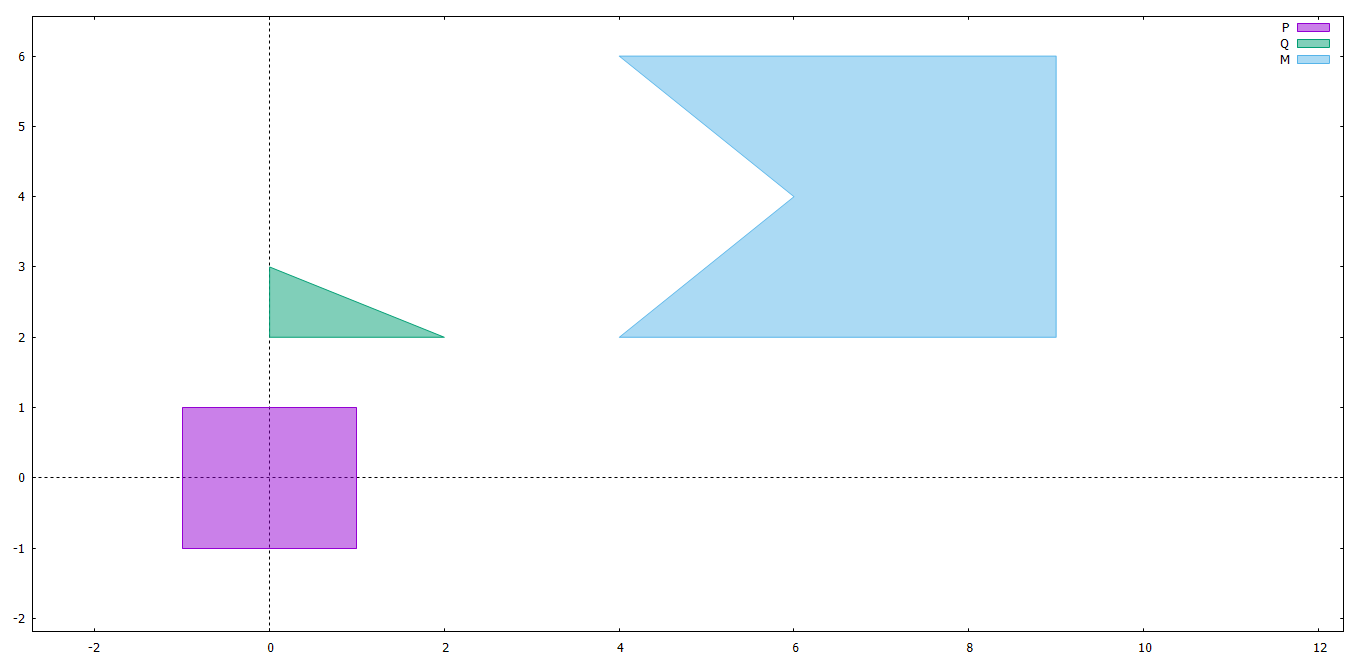
\includegraphics[width=1.0\textwidth]{game}
    \caption{Пример игры}
    \label{fig:game}
\end{figure}

Рассмотрим игру на прожутке $[0, 5]$ с шагом $\Delta = 1$.

В результате работы программы, 
получили пять сечений максимального стабильного моста.
Все они изображены на рисунке \ref{fig:bridge}.

\begin{figure}
    \centering
    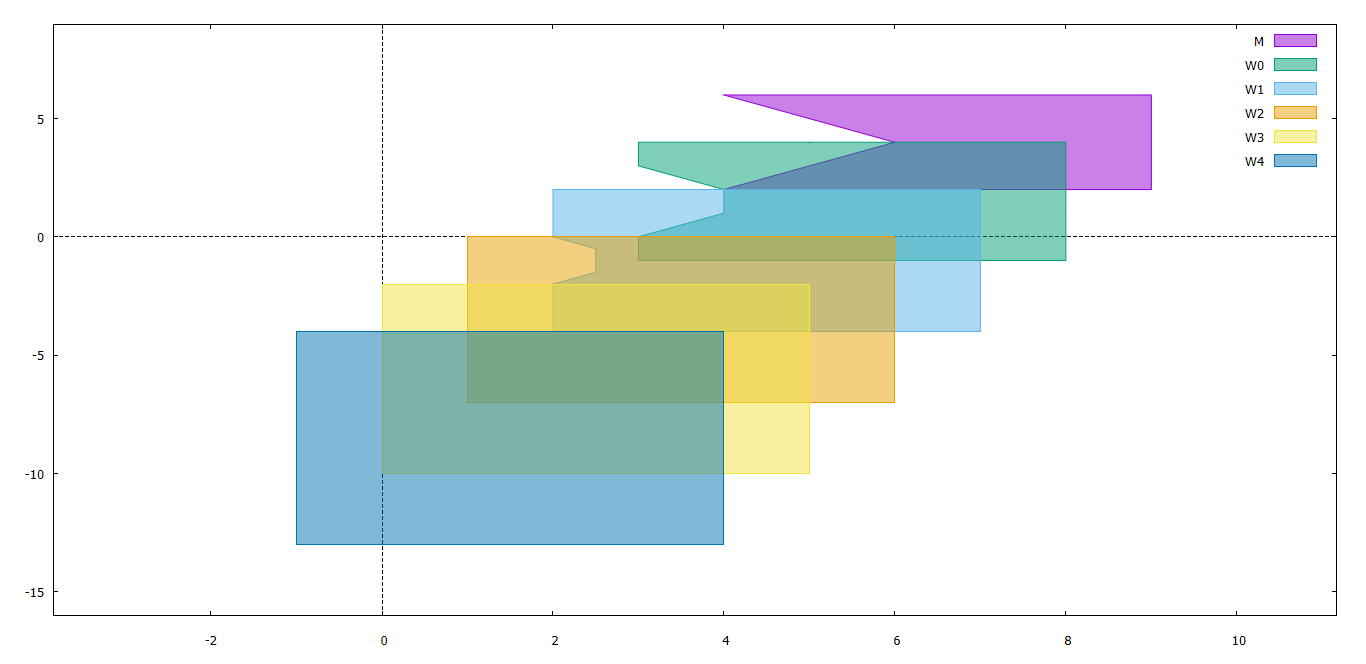
\includegraphics[width=1.0\textwidth]{bridge}
    \caption{Стабильный мост}
    \label{fig:bridge}
\end{figure}